  %% ACM sigconf: full two-column research report (nonacm). Build:  pdflatex bimodal_report  (x2)
  \documentclass[sigconf,nonacm]{acmart}
  \usepackage{amsmath}
  \usepackage{booktabs}
  \usepackage[english]{babel}
  \usepackage{balance}
  \usepackage{microtype}
  \usepackage{graphicx}
  % Self-contained for Overleaf: all generated evaluation values are inlined below.
  % Per-class qualitative thumbnails live under eval_output/qual_images/ ; upload
  % that folder to Overleaf alongside this file to render Table~\ref{tab:qualimages}.
  \graphicspath{{eval_output/}{./}}

  % Course submission: no permission footnote
  \renewcommand\footnotetextcopyrightpermission[1]{}
  \settopmatter{printacmref=false,printfolios=true}

  % --- title & authors (edit names/emails before submission if desired) ---
  \title[Bimodal Affective Alignment]{Bimodal Affective Alignment: Enhancing Conversational Empathy through Textual and Facial Fusion}

  \author{Sainadth Pagadala}
  \email{spagadala1@islander.tamucc.edu}
  \affiliation{%
    \department{College of Engineering and Computer Science}
    \institution{Texas A\&M University--Corpus Christi}
    \city{Corpus Christi}
    \state{TX}
    \postcode{78412}
    \country{USA}}
  \author{Vishakan Umapathy}
  \email{vumapathy@islander.tamucc.edu}
  \affiliation{%
    \department{College of Engineering and Computer Science}
    \institution{Texas A\&M University--Corpus Christi}
    \city{Corpus Christi}
    \state{TX}
    \postcode{78412}
    \country{USA}}
  \author{Minhua Huang}
  \authornote{Course instructor and project advisor.}
  \email{minhua.huang@tamucc.edu}
  \affiliation{%
    \department{College of Engineering and Computer Science}
    \institution{Texas A\&M University--Corpus Christi}
    \city{Corpus Christi}
    \state{TX}
    \postcode{78412}
    \country{USA}}
  \renewcommand{\shortauthors}{Pagadala, Umapathy, and Huang}

  % CCS 2012
  \begin{CCSXML}
  <ccs2012>
  <concept>
    <concept_id>10003120.10003121</concept_id>
    <concept_desc>Human-centered computing~Human computer interaction (HCI)</concept_desc>
    <concept_significance>500</concept_significance>
  </concept>
  <concept>
    <concept_id>10010147.10010257.10010293.10010294</concept_id>
    <concept_desc>Computing methodologies~Neural networks</concept_desc>
    <concept_significance>300</concept_significance>
  </concept>
  </ccs2012>
  \end{CCSXML}
  \ccsdesc[500]{Human-centered computing~Human computer interaction (HCI)}
  \ccsdesc[300]{Computing methodologies~Neural networks}

  \keywords{affective computing, emotion recognition, multimodal fusion, GoEmotions, FER, FLAN-T5, dialogue}

  \begin{document}
  \begin{abstract}
  Conversational systems that read only one channel of human affect often misread the situation: text can hide what a person is feeling, and a face can contradict the words. This work builds and evaluates a bimodal pipeline that listens to both at once. A RoBERTa text classifier (fine-tuned on GoEmotions) and a ResNet-50 face classifier (FER2013-aligned) each emit a seven-way affect distribution, and a single trust weight $\alpha\in[0,1]$ fuses them via
  $b^*=\arg\max_k\bigl(\alpha P_\text{text}(k)+(1\!-\!\alpha)P_\text{face}(k)\bigr)$.
  The fused class together with the user's utterance feeds FLAN--T5, which produces a short empathetic reply. A Streamlit interface exposes both probability vectors, the fused decision, an explicit affective-dissonance flag, and per-stage timings, so a reviewer can see -- not just trust -- how the system is reasoning. We report unimodal and fused accuracy on the full GoEmotions and FER2013 test splits, a FER2013 fine-tune that lifts visual top-1 from 23.1\% to 68.5\%, real-image and synthetic dissonance evaluations, and a latency breakdown. Affect inference takes about 38\,ms on Apple MPS -- well inside the 400\,ms Doherty threshold -- while end-to-end response generation with FLAN--T5 (base) lands at 942\,ms.
  \end{abstract}

  \maketitle

  \section{Introduction}
  \subsection{Problem and motivation}
  When a dialogue system has to infer affect from text alone it is easy to fool: a sarcastic remark looks happy on the surface, a polite ``I'm fine'' hides distress, and a deadpan one-liner gives almost no signal at all. Vision alone has the symmetric weakness -- the same neutral face appears in good lighting, bad lighting, off-axis, or partly occluded. In either case the system has to guess, and a wrong guess in the empathy loop erodes user trust quickly~\cite{card1983human}. Reading both channels at once, when they are available, gives the model a second opinion and -- equally important -- a way to flag the cases where the two opinions disagree.

  \subsection{Related work}
  Facial expression recognition and text-based emotion classification are each mature on their own. What is comparatively rare at course scale is a tight \emph{coupling} of the two in a shared seven-class label space with an exposed trust weight. We borrow the GoEmotions corpus of Demszky et~al.~\cite{demeszky2020goemotions} for text, the FER2013-style ResNet recipe of Goodfellow et~al.~\cite{goodfellow2013challenges} for vision, and the instruction-tuned T5 family of Chung et~al.~\cite{chung2022scaling} for the empathetic response. Latency expectations are framed against the 400\,ms Doherty interaction threshold from Card, Newell, and Moran~\cite{card1983human}.

  \subsection{Approach and contributions}
  The pipeline mirrors the course architecture (Fig.~\ref{fig:pipeline}). A transformer text sensor (RoBERTa fine-tuned on GoEmotions~\cite{demeszky2020goemotions}) emits $P_\text{text}$ over the seven FER classes; a ResNet-50 face sensor~\cite{goodfellow2013challenges} emits $P_\text{face}$ over the same seven classes; a late fusion (Eq.~\ref{eq:main}) blends them with a trust weight~$\alpha$; and a FLAN--T5 generator~\cite{chung2022scaling} turns the fused class into a short empathetic reply. We make five concrete contributions: (1) a deterministic surjection from the 28 GoEmotions labels into the 7 FER classes; (2) an end-to-end Streamlit demo that exposes every intermediate signal so a reviewer can probe the system rather than just consume its output; (3) a separate FER2013 fine-tuning workflow that takes the face branch from a near-chance 23.1\% to 68.5\% top-1 without altering the deployed code path; (4) scripted ablation, $\alpha$-sensitivity, dissonance, and latency benchmarks tied to the same shared evaluation harness; and (5) an honest discussion of the places each component still breaks.

  \begin{figure*}[t]
  \centering
  \fbox{%
  \parbox{0.96\textwidth}{\centering\footnotesize\sf
  \textbf{Input:} user utterance $U$, image frame $I$.\\[0.7em]
  \begin{tabular}{c@{\hspace{3em}}c}
    $U \;\xrightarrow{\;\text{\texttt{RoBERTa}--GoEmotions}\;}\; P_\text{text}\!\in\!\mathbb{R}^{7}$ &
    $I \;\xrightarrow{\;\text{ResNet--50 (7-way FER)}\;}\; P_\text{face}\!\in\!\mathbb{R}^{7}$
  \end{tabular}\\[0.6em]
  $(P_\text{text},\,P_\text{face}) \;\xrightarrow{\;\text{late fusion, trust }\alpha\;}\; b^{*}\;\text{(Eq.~\ref{eq:main})}\;\xrightarrow{\;\text{FLAN--T5}\;}\; R\;\text{(empathetic reply)}$%
  }
  }
  \Description{Block diagram of the bimodal affective alignment pipeline. The user utterance U feeds RoBERTa fine-tuned on GoEmotions, producing a 7-way text probability vector P_text. The image frame I feeds a 7-way ResNet-50 face emotion classifier, producing P_face. Both probability vectors are combined by the late-fusion equation b* = argmax (alpha P_text + (1 - alpha) P_face). The fused FER-7 class b* and the original utterance U are passed to FLAN-T5, which emits an empathetic reply R.}
  \caption{Bimodal affective processing pipeline. Both branches align to the same FER\texorpdfstring{$7$}{\,7} label set before fusion.}
  \label{fig:pipeline}
  \end{figure*}

  \section{Formulation}
  Let the FER-7 label index be $k\in\{1,\ldots,7\}$. The text branch produces $P_\text{text}$ and the face branch produces $P_\text{face}$; after per-branch normalization both live on the probability simplex. We combine them by a late-fusion convex blend and read out the discrete decision via an $\arg\max$:
  \begin{equation}
    b^* = \arg\max_{k} \left( \alpha\, P_\text{text}(k) + (1-\alpha)\, P_\text{face}(k) \right), \quad \alpha\in[0,1].
    \label{eq:main}
  \end{equation}
  Setting $\alpha\!=\!1$ recovers the text-only ablation, $\alpha\!=\!0$ recovers the face-only ablation, and $\alpha\!=\!0.5$ is the balanced setting we treat as the system default. Sweeping $\alpha$ across $[0.2,0.8]$ probes how brittle the fused decision is to the trust setting. We flag a sample as showing \emph{affective dissonance} whenever $\arg\max P_\text{text}\neq\arg\max P_\text{face}$; this flag is what the Streamlit interface surfaces to the user as a coloured badge.

  \section{Method}
  \subsection{Mapping 28 GoEmotions labels to FER\texorpdfstring{$7$}{\,7}}
  GoEmotions ships with 28 fine-grained emotion strings, while the visual branch can only resolve seven. We collapse the 28 to the 7 with a hand-coded surjection that lives in the codebase as a single Python dictionary: every GoEmotions string maps to exactly one of \{\,Angry, Disgust, Fear, Happy, Sad, Surprise, Neutral\,\}. Because GoEmotions is multilabel and uses sigmoid scores, we \emph{sum} the sigmoid mass landing in each FER-7 bin and renormalize to a proper distribution; this keeps the relative confidence of fine-grained labels (e.g., \emph{annoyance} adding to \emph{anger}) when several map to the same bin.

  \subsection{Language model}
  The text sensor is the public RoBERTa-base GoEmotions checkpoint \texttt{SamLowe/roberta-base-go\_emotions} on HuggingFace, which corresponds to the assignment's ``BERT/RoBERTa on GoEmotions'' requirement and lets us avoid retraining a 28-way head from scratch.

  \subsection{Visual model and preprocessing}
  The face branch is a 7-way ResNet-50 head that consumes a $224\!\times\!224$ RGB input with FER/AffectNet-style mean normalization. The deployed app loads \texttt{ElenaRyumina/face\_emotion\_recognition} as the baseline checkpoint, which is convenient because it is publicly available and works out of the box on near-frontal RGB faces. It is also where most of our visual-branch error budget lives, because FER2013 test images are 48$\!\times\!48$ grayscale faces upscaled to 224$\!\times\!224$ -- a noticeable domain shift away from the AffectNet distribution this checkpoint was trained on. To quantify and partially close that gap we also fine-tune the same head on the \texttt{AutumnQiu/fer2013} train split (Table~\ref{tab:finetune}). The fine-tuned weights are evaluated independently of the deployed path so the baseline numbers in this report stay reproducible.

  \subsection{Empathetic response generation}
  Once the fused class $b^{*}$ is decided, the user utterance $U$ and a verbalized form of $b^{*}$ are passed to FLAN--T5 (base, 220M parameters) under a deterministic instruction prompt (full prompt in Section~\ref{sec:gen-samples}). Only $U$ and the FER-7 class string flow into the prompt, following the assignment specification; the probability vectors themselves are not exposed to the language model.

  \section{System Implementation}\label{sec:Implementation}
  The implementation is Python on top of PyTorch, HuggingFace \texttt{transformers} and \texttt{datasets}, Streamlit, Pillow, and NumPy. The interface accepts either a webcam frame or an uploaded image, presents the user with a slider for~$\alpha$, three side-by-side probability bar charts (text, face, fused), a dissonance badge, the generated empathetic reply, and a timing panel that breaks the latency down by stage (text, face, fusion, FLAN--T5, total). The same codebase ships scripts that reproduce every number in this report -- congruent unimodal/fused benchmarks, synthetic and real-image dissonance evaluations, the latency study, the qualitative tables, and the FER2013 fine-tune. All of these run independently of the demo app so that toggling between the baseline and fine-tuned visual checkpoints does not require any change to the deployed code path.

  \section{Experiments, HCI evaluation, and limitations}

  \subsection{Quantitative benchmark (FER\texorpdfstring{$7$}{\,7} top-1)}
  Three modes are reported, mirroring the course handout. The \emph{text-only} setting runs the single-label slice of the GoEmotions test set with each gold label mapped into FER-7. The \emph{image-only} setting runs the full FER2013 test split through the visual branch in isolation. The \emph{bimodal} setting pairs each FER2013 test image with a fixed emotion-matched template sentence and fuses the two probability vectors at $\alpha\!=\!0.5$, exactly as in Eq.~\ref{eq:main}. The lower two rows in Table~\ref{tab:results} are an ablation on those same image-plus-template pairs: they report what the text branch and the face branch each say on their own, so the fused row can be read against its own components rather than against an unrelated reference. The reported run uses every available single-label GoEmotions test example ($n\!=\!4590$) and the full FER2013 test split ($n\!=\!3589$). To reproduce:
  \begin{quote}\small\noindent
  \texttt{python scripts/run\_evaluation.py}\\
  \texttt{\hspace*{1em} --limit 5000 --out docs/eval\_output}
  \end{quote}

  \begin{table*}[t]
    \centering
    \small
    \caption{Top-1 FER$7$ accuracy (run: $n$ limited to 5000 per sub-task; the available test sets have 4590 GoEmotions single-label and 3589 FER2013 examples; $\alpha\!=\!0.5$ for fusion). \emph{Text:} GoEmotions test, single\nobreakdash label (mapped to FER$7$). \emph{Image:} \texttt{AutumnQiu/fer2013}. \emph{Bimodal:} one emotion\nobreakdash matched template per FER class; fusion per Eq.~\ref{eq:main}. Lower two rows: text-only and image-only \emph{branches} on the same bimodal pairs (ablation).}
    \label{tab:results}
    \begin{tabular}{@{}lcc@{}}
      \toprule
      \textbf{Setting} & \textbf{$n$} & \textbf{Acc. (\%)} \\
      \midrule
      Text--only (GoEmotions) & 4590 & 69.7 \\
      Image--only (FER2013) & 3589 & 23.1 \\
      Text$+$image fused & 3589 & 81.6 \\
      \midrule
      Text branch only (same pairs) & 3589 & 82.6 \\
      Image branch only (same pairs) & 3589 & 23.1 \\
      \bottomrule
    \end{tabular}
  \end{table*}

  \subsection{Fine-tuning the visual branch}
  The default visual checkpoint is fine for a live demo, but it is clearly the weakest part of the pipeline on FER2013 test data: an AffectNet-trained model asked to score 48$\!\times\!48$ grayscale frames is operating well outside its training distribution. We therefore fine-tuned the same ResNet-50 head on the \texttt{AutumnQiu/fer2013} train split with a held-out validation slice and standard cross-entropy. Table~\ref{tab:finetune} shows the result: full-test top-1 accuracy moves from 23.1\% to 68.5\%, almost a three-fold improvement and roughly the difference between near-chance and a usable face signal. We deliberately keep the fine-tuned weights as a separate checkpoint from the deployed demo so that every baseline number in this report stays reproducible without any extra setup; \texttt{scripts/eval\_fer\_checkpoint.py} loads the new file directly when the reader wants to verify the fine-tuned numbers.

  \begin{table}[t]
    \centering
    \small
    \caption{FER2013 test accuracy before and after visual fine-tuning ($n=3589$).}
    \label{tab:finetune}
    \begin{tabular}{@{}lcc@{}}
      \toprule
      \textbf{Visual checkpoint} & \textbf{$n$} & \textbf{Acc. (\%)} \\
      \midrule
      Baseline HF ResNet--50 & 3589 & 23.1 \\
      FER2013 fine-tuned ResNet--50 & 3589 & 68.5 \\
      \bottomrule
    \end{tabular}
  \end{table}

  \subsection{Dissonance and trust weight}
  ``Dissonance'' here is the case in which the text and the face disagree about what the user feels. We probe it two complementary ways. The real-image probe pairs every FER2013 test image with a deliberately mismatched template sentence and treats the FER2013 label as the intended affect; the fused decision should ideally recover that intended label, but the baseline face branch is only 23.1\% accurate on FER2013, so most of the time the system follows the misleading text rather than the noisy face. The synthetic probe replaces the face branch with a one-hot vector for the intended class, which isolates the fusion arithmetic from any face-classifier noise: when one of the two inputs is perfect, $\alpha\!=\!0.5$ should -- and does -- recover the intended class even though the other input is wrong by construction. Table~\ref{tab:dissonance} lists both. We treat the real-image row as the honest result and the synthetic row as a sanity check on the fusion rule itself.

  \begin{table*}[t]
    \centering
    \small
    \caption{Dissonant evaluation. Real-image rows use actual FER2013 images on the full test split ($n\!=\!3589$); synthetic rows use one-hot face vectors over a 100-row controlled grid. In both cases, text is intentionally mismatched with the intended class via $j\!=\!(y\!+\!1\!+\!(k\bmod 6))\bmod 7$.}
    \label{tab:dissonance}
    \begin{tabular}{@{}lcccc@{}}
      \toprule
      \textbf{Dissonant setting} & \textbf{$n$} & \textbf{$\alpha=1$ text} & \textbf{$\alpha=0.5$ fused} & \textbf{$\alpha=0$ face} \\
      \midrule
      Real FER2013 images + mismatched template text   & 3589 & 4.0\%  & 4.3\%   & 23.1\% \\
      Synthetic one-hot face + mismatched template text & 100  & 3.0\%  & 100.0\% & 100.0\% \\
      \bottomrule
    \end{tabular}
  \end{table*}

  Table~\ref{tab:qualdissimages} drills into the real-image dissonant setting with the first 10 FER2013 test images -- the same indices that contribute to the aggregate row above. The mismatched-text class~$j$ is fixed by the row index via $j = (y + 1 + (k\bmod 6)) \bmod 7$, so every row has a different gold/text pairing and we are not cherry-picking. Three patterns jump out. The text branch follows the planted misdirection on all 10 rows, which is consistent with the $\sim$4\% aggregate $\alpha\!=\!1$ accuracy. The face branch -- still the baseline AffectNet checkpoint here -- collapses to \emph{Happy} on 7 of 10 rows, which is the visual-branch domain shift we describe in Section~\ref{sec:failmodes}. And the fused decision essentially tracks the text branch because the gold-versus-mismatch distinctions (Angry vs.\ Disgust, Sad vs.\ Surprise, etc.) are well below the resolution of a 23\%-accurate face signal. We revisit the same 10 rows with the fine-tuned face branch in Section~\ref{sec:finetuned}; the two tables share image indices so the reader can flip between them and compare the two visual backbones row by row.

\begin{table*}[t]
  \small
  \centering
  \caption{Dissonant qualitative cases. Real FER2013 test image (gold class) paired with the congruent template text of a deliberately mismatched FER-7 class. We list the predicted FER-7 class at $\alpha\!=\!1$ (text-only, expected to match the text class), $\alpha\!=\!0.5$ (fused), and $\alpha\!=\!0$ (face-only, expected to match the gold class) using the baseline ElenaRyumina ResNet-50 face branch. A check mark indicates the prediction matches the \emph{gold} face class. Local hit rates over these 10 rows: $\alpha\!=\!1$ 0/10, $\alpha\!=\!0.5$ 0/10, $\alpha\!=\!0$ 2/10.}
  \label{tab:qualdissimages}
  \setlength{\tabcolsep}{4pt}
  \renewcommand{\arraystretch}{1.15}
  \begin{tabular}{@{}c l l p{0.40\textwidth} c c c@{}}
    \toprule
    \textbf{Image} & \textbf{Gold} & \textbf{Text class} & \textbf{Mismatched user text $U$} & \textbf{$\alpha\!=\!1$} & \textbf{$\alpha\!=\!0.5$} & \textbf{$\alpha\!=\!0$} \\
    \midrule
    \includegraphics[width=1.4cm]{qual_dissonant_images/00_angry_vs_disgust.png} & Angry & Disgust & That is completely disgusting, I feel revolted and sickened by what I am seeing. & Disgust & Disgust & Happy \\
    
\includegraphics[width=1.4cm]{qual_dissonant_images/01_surprise_vs_angry.png} & Surprise & Angry & I am absolutely furious and enraged; this is unacceptable and I will not stand for it. & Angry & Angry & Angry \\
    
\includegraphics[width=1.4cm]{qual_dissonant_images/02_neutral_vs_fear.png} & Neutral & Fear & I am terrified and panicked; I feel deep fear and anxiety about this situation right now. & Fear & Fear & Happy \\
    \includegraphics[width=1.4cm]{qual_dissonant_images/03_sad_vs_disgust.png} & Sad & Disgust & That is completely disgusting, I feel revolted and sickened by what I am seeing. & Disgust & Disgust & Happy \\
    \includegraphics[width=1.4cm]{qual_dissonant_images/04_fear_vs_angry.png} & Fear & Angry & I am absolutely furious and enraged; this is unacceptable and I will not stand for it. & Angry & Angry & Happy \\
    \includegraphics[width=1.4cm]{qual_dissonant_images/05_angry_vs_neutral.png} & Angry & Neutral & It is a normal quiet day; I feel pretty neutral and nothing in particular is happening to me. & Happy & Happy & Happy \\
    
\includegraphics[width=1.4cm]{qual_dissonant_images/06_sad_vs_surprise.png} & Sad & Surprise & I am so shocked and surprised I can barely process what just happened, this is incredible. & Surprise & Surprise & Angry \\
    \includegraphics[width=1.4cm]{qual_dissonant_images/07_happy_vs_surprise.png} & Happy & Surprise & I am so shocked and surprised I can barely process what just happened, this is incredible. & Surprise & Surprise & Happy \checkmark \\
    
\includegraphics[width=1.4cm]{qual_dissonant_images/08_angry_vs_happy.png} & Angry & Happy & I am overjoyed and delighted; I could not be happier with this amazing wonderful news today! & Happy & Happy & Happy \\
    \includegraphics[width=1.4cm]{qual_dissonant_images/09_happy_vs_angry.png} & Happy & Angry & I am absolutely furious and enraged; this is unacceptable and I will not stand for it. & Angry & Angry & Happy \checkmark \\
    \bottomrule
  \end{tabular}
\end{table*}

  \subsection{Trust-weight $\alpha$ sensitivity}
  Eq.~\ref{eq:main} is a one-parameter family of decision rules, and three points along it are operationally meaningful: $\alpha\!=\!1$ (text only), $\alpha\!=\!0$ (face only), and the balanced $\alpha\!=\!0.5$. We adopt $\alpha\!=\!0.5$ as the system default for two reasons. First, on the matched bimodal benchmark in Table~\ref{tab:results} the fused decision scores 81.6\% top-1, only one point below the 82.6\% text branch on the same pairs -- a small price for a face-aware decision rule. Second, the dissonant evaluations in Table~\ref{tab:dissonance} show that $\alpha\!=\!0.5$ inherits whichever branch is the more confident: with a one-hot synthetic face vector it reaches 100\% even when the text input is wrong by construction (3\%), and with the noisy baseline face it stays bounded by the weak face signal (4.3\% vs.\ 23.1\%). Put another way, $\alpha$ is meant to be an interpretable HCI knob, not a hyperparameter to tune on a held-out set, so we expose it on the Streamlit sidebar instead of optimizing it away. A reviewer who wants to probe the same input under different trust regimes can simply slide $\alpha$ and watch the dissonance badge.

  \subsection{Latency and HCI review}
  The deployed app reports per-stage timings, and we replicate them in a scripted benchmark on Apple MPS using 3 warm-up runs followed by 15 timed runs over a fixed utterance and synthetic face frame. The affect subtotal -- text plus face plus the fusion arithmetic -- finishes in roughly 38\,ms, well under the 400\,ms Doherty threshold from the HCI literature, so a user holding a slider on $\alpha$ sees the bar charts update with no perceptible lag. End-to-end latency including FLAN--T5 (base) generation rises to 942\,ms (Table~\ref{tab:latency}); generation dominates because we use deterministic beam search with $n_\text{beams}\!=\!4$ on a 220M-parameter model running on a laptop GPU. In a deployed product, the response would be streamed token-by-token so that the user perceives a sub-400\,ms onset even though the full message lands later. We do not claim a formal participant Likert study; instead, we offer per-class qualitative cases on real FER2013 images (Table~\ref{tab:qualimages}), the actual FLAN--T5 replies that go with them (Table~\ref{tab:qualresponses}), expert-review dissonant examples in the course handout format (Table~\ref{tab:qual}), and a ready-to-run Likert template at \texttt{docs/HCI\_STUDY\_TEMPLATE.md} for future participants.

  \begin{table}[t]
    \centering
    \small
    \caption{Latency benchmark on Apple MPS (15 timed runs after 3 warm-up runs). FLAN--T5 base, beam search (4 beams), $\geq$18 / $\leq$128 new tokens.}
    \label{tab:latency}
    \begin{tabular}{@{}lcc@{}}
      \toprule
      \textbf{Stage} & \textbf{Mean (ms)} & \textbf{Std. dev. (ms)} \\
      \midrule
      Text model            &  18.9 &  3.1 \\
      Face model            &  19.4 &  4.0 \\
      Fusion                &   0.1 &  0.0 \\
      Affect subtotal       &  38.4 &  --  \\
      FLAN--T5 (base) gen.  & 903.9 & 69.7 \\
      End-to-end            & 942.2 & 67.7 \\
      \bottomrule
    \end{tabular}
  \end{table}

  \subsection{Per-class qualitative cases (real FER2013 images)}
  Table~\ref{tab:qualimages} samples one real FER2013 test image per FER-7 gold class and pairs it with the matching congruent template text. We then read out the predicted FER-7 class at $\alpha\!=\!1$ (text only), $\alpha\!=\!0.5$ (fused), and $\alpha\!=\!0$ (face only) using the baseline ResNet-50. Two patterns stand out. The face branch is unreliable on FER2013: it misclassifies 5 of the 7 images on its own, which is the per-row picture behind the 23.1\% aggregate in Table~\ref{tab:results}. The text branch, on the other hand, pulls the fused decision toward the correct gold class on 6 of 7 cases. The single failure is the Neutral row, where the template text itself contains positive-sounding language (``\texttt{feel pretty neutral}''), and the GoEmotions head reads it as Happy -- the kind of subtle text-side mistake the trust weight $\alpha$ is meant to surface rather than hide.

  \begin{table*}[t]
    \small
    \centering
    \caption{Per-class qualitative cases. One real FER2013 test image per FER-7 gold class, paired with the emotion-matched congruent template as text. We list the predicted FER-7 class at $\alpha\!=\!1$ (text-only), $\alpha\!=\!0.5$ (fused), and $\alpha\!=\!0$ (face-only) using the baseline ElenaRyumina ResNet-50 face branch on a 48$\times$48 grayscale FER2013 frame.}
    \label{tab:qualimages}
    \setlength{\tabcolsep}{4pt}
    \renewcommand{\arraystretch}{1.15}
    \begin{tabular}{@{}c l p{0.46\textwidth} c c c@{}}
      \toprule
      \textbf{Image} & \textbf{Gold} & \textbf{User text $U$} & \textbf{$\alpha\!=\!1$} & \textbf{$\alpha\!=\!0.5$} & \textbf{$\alpha\!=\!0$} \\
      \midrule
      \includegraphics[width=1.4cm]{qual_images/0_angry.png} & Angry & I am absolutely furious and enraged; this is unacceptable and I will not stand for it. & Angry & Angry & Happy \\
      
\includegraphics[width=1.4cm]{qual_images/1_disgust.png} & Disgust & That is completely disgusting, I feel revolted and sickened by what I am seeing. & Disgust & Disgust & Happy \\
      \includegraphics[width=1.4cm]{qual_images/2_fear.png} & Fear & I am terrified and panicked; I feel deep fear and anxiety about this situation right now. & Fear & Fear & Happy \\
      \includegraphics[width=1.4cm]{qual_images/3_happy.png} & Happy & I am overjoyed and delighted; I could not be happier with this amazing wonderful news today! & Happy & Happy & Happy \\
      \includegraphics[width=1.4cm]{qual_images/4_sad.png} & Sad & I feel heartbroken, deeply sad, and I could cry; everything feels gray and empty to me. & Sad & Sad & Happy \\
      
\includegraphics[width=1.4cm]{qual_images/5_surprise.png} & Surprise & I am so shocked and surprised I can barely process what just happened, this is incredible. & Surprise & Surprise & Angry \\
      
\includegraphics[width=1.4cm]{qual_images/6_neutral.png} & Neutral & It is a normal quiet day; I feel pretty neutral and nothing in particular is happening to me. & Happy & Happy & Happy \\
      \bottomrule
    \end{tabular}
  \end{table*}

  \subsection{Generated response samples}\label{sec:gen-samples}
  Once the fused class $b^{*}$ is decided, the user utterance $U$ and the FER-7 class string for $b^{*}$ are handed to FLAN--T5 (base, 220M) under a deterministic instruction prompt. Crucially, only $U$ and $b^{*}$ flow into the prompt -- the probability vectors themselves are never exposed to the language model -- which keeps the response stage in line with the assignment specification. The prompt is, lightly abbreviated:
  \begin{quote}\small\itshape
  ``You are an empathetic counsellor talking to a user. Reply to the user in 2 short sentences using the word \emph{you} at least once. Acknowledge that they feel \texttt{<descriptor(b*)>}, validate the feeling, then ask one short open question. Do NOT repeat the user's sentence verbatim and do NOT speak in the first person; address the user.\\ User said: \texttt{<U>}\\ Inferred emotion: \texttt{<b*>}.\\ Empathetic reply (begin with ``It sounds like'' or ``I hear''):''
  \end{quote}
  The prompt verbalizes $b^{*}$ through a fixed seven-entry descriptor table (e.g.\ \texttt{Sad}\,$\to$\,``sad and discouraged'') so that the small base model attends to a richer adjective phrase rather than a bare class label. Decoding is deterministic beam search ($n_\text{beams}\!=\!4$, no-repeat 3-grams, repetition penalty 1.6, between 18 and 128 new tokens, no sampling). Table~\ref{tab:qualresponses} lists the actual reply $R$ for each row of Table~\ref{tab:qualimages}. Five of the seven rows produce a clean second-person acknowledgement plus a reflective follow-up question, which is what the prompt asks for. The Sad row exposes a known habit of FLAN--T5 base, where it slips into a multiple-choice answer format, and the Surprise row paraphrases $U$ instead of asking a real question. We read these as limitations of the 220M backbone, not of the alignment pipeline; swapping in any 1B-class instruction-tuned model is a one-line change in \texttt{response\_synthesizer.py} and would improve generation quality without affecting any of the affect-alignment numbers above.

  \begin{table*}[t]
    \small
    \centering
    \caption{FLAN--T5 (base) empathetic replies $R$ generated for the per-class qualitative cases of Table~\ref{tab:qualimages}. Decoding is deterministic beam search; only $U$ and the fused FER-7 class label $b^{*}$ feed the prompt.}
    \label{tab:qualresponses}
    \setlength{\tabcolsep}{4pt}
    \renewcommand{\arraystretch}{1.2}
    \begin{tabular}{@{}l l p{0.72\textwidth}@{}}
      \toprule
      \textbf{Gold} & \textbf{Fused $b^{*}$} & \textbf{Generated empathetic reply $R$} \\
      \midrule
      Angry    & Angry    & I hear that you are angry. What do you mean by ``I will not stand for it''? \\
      Disgust  & Disgust  & Is it a bad thing to be seeing what you're seeing, or is it disgusting? \\
      Fear     & Fear     & I hear you are scared and anxious about this situation right now. What is the cause of your fear? \\
      Happy    & Happy    & I hear that you are happy and excited. What do you mean by ``overjoyed''? \\
      Sad      & Sad      & Is everything gray and empty to me? (i) Yes. (ii) No. \\
      Surprise & Surprise & I hear that you're so shocked and surprised I can barely process what just happened, this is incredible. \\
      Neutral  & Happy    & Is it a normal quiet day, or is there something in particular happening to me? \\
      \bottomrule
    \end{tabular}
  \end{table*}

  \subsection{Failure modes}\label{sec:failmodes}
  Two qualitative failure modes show up in our data, and they are worth naming explicitly. The first is \textbf{visual-branch domain shift}: the baseline ResNet-50 head was trained on color, near-frontal, AffectNet-style faces, and is then asked to score 48$\!\times\!48$ grayscale FER2013 frames that are upscaled to 224$\!\times\!224$. Predictably, the face branch defaults to \emph{Happy} on 5 of the 7 qualitative cases in Table~\ref{tab:qualimages} and lands at a 23.1\% face-only top-1 across the full FER2013 test split (Table~\ref{tab:dissonance}). Fine-tuning on FER2013 closes most of this gap, taking face-only top-1 from 23.1\% to 68.5\% (Table~\ref{tab:finetune}). The second is \textbf{text-branch sentiment leak}: the GoEmotions head reacts to surface cue words rather than to the propositional content of $U$. The Neutral congruent template -- ``\textit{It is a normal quiet day; I feel pretty neutral and nothing in particular is happening to me}'' -- is classified as Happy because of the phrase ``\textit{feel pretty}''. This is a known weakness of single-utterance sentiment classifiers, and it is exactly the failure mode the trust-weight $\alpha$ is designed to surface: a reviewer who lowers $\alpha$ on this row sees the face branch (also Happy here) confirm the text decision, while raising $\alpha$ would not rescue the Neutral label either. The mistake is honest and visible, not silent.

  \begin{table*}[t]
    \small
    \centering
    \caption{Expert-review dissonant examples following the course handout format.}
    \label{tab:qual}
    \setlength{\tabcolsep}{4pt}
    \begin{tabular}{@{}p{0.20\textwidth}p{0.12\textwidth}p{0.12\textwidth}p{0.50\textwidth}@{}}
      \toprule
      User input $U$ & Text (argmax) & Face (e.g.\ argmax) & Bimodal empathetic $R$ (intent) \\
      \midrule
      ``I'm fine, really.'' & Neutral & Sad & ``I hear you, but you look a bit troubled. Is something on your mind?'' \\
      ``I can't believe it!'' & Surprise & Happy & ``That sounds like big news---you seem excited; I am glad for you.'' \\
      ``Yeah, great job.'' & Happy & Angry & ``I sense some frustration despite the positive words. What happened?'' \\
      \bottomrule
    \end{tabular}
  \end{table*}

  \subsection{Fine-tuned model results}\label{sec:finetuned}
  Every preceding table in this report uses the \emph{baseline} ResNet-50 face branch -- the public AffectNet-trained \texttt{ElenaRyumina/face\_emotion\_recognition} checkpoint -- so that the main numbers correspond exactly to the deployed default app. This subsection re-runs the same evaluations with the FER2013 fine-tuned face branch swapped in (Table~\ref{tab:finetune}) so the reader can see how each downstream metric changes once the visual branch is corrected for the FER2013 domain shift.

  \emph{Bimodal congruent (matched template text + real FER2013 image).} Re-running the unimodal/bimodal benchmark of Table~\ref{tab:results} with the fine-tuned face branch substituted in (\texttt{scripts/run\_evaluation.py --finetune-ckpt}) gives Table~\ref{tab:resultsft}. The text branch is unchanged, as expected. The image branch tracks the FER2013 image-only fine-tune from Table~\ref{tab:finetune} (23.1\,\%~$\to$~68.5\,\%). And the fused $\alpha\!=\!0.5$ score climbs from 81.6\,\% to \textbf{87.8\,\%} -- now clearly above the 82.6\,\% text branch on the same pairs. This is the first regime in which adding the face actually \emph{helps} the fused decision rather than gently dragging it down.

  \begin{table*}[t]
    \centering
    \small
    \caption{Top-1 FER$7$ accuracy with the \textbf{fine-tuned} ResNet-50 face branch substituted in (companion to Table~\ref{tab:results}; same evaluation protocol, $n$ limited to 5000 per sub-task; $\alpha\!=\!0.5$ for fusion).}
    \label{tab:resultsft}
    \begin{tabular}{@{}lcc@{}}
      \toprule
      \textbf{Setting} & \textbf{$n$} & \textbf{Acc. (\%)} \\
      \midrule
      Text--only (GoEmotions)                   & 4590 & 69.7 \\
      Image--only (FER2013, fine-tuned ResNet)  & 3589 & 68.5 \\
      Text$+$image fused                        & 3589 & \textbf{87.8} \\
      \midrule
      Text branch only (same pairs)             & 3589 & 82.6 \\
      Image branch only (same pairs)            & 3589 & 68.5 \\
      \bottomrule
    \end{tabular}
  \end{table*}

  \emph{Real-image dissonance, aggregate.} Re-running \texttt{scripts/eval\_dissonant\_fer2013.py --finetune-ckpt} on the full FER2013 test split ($n\!=\!3589$ deliberately mismatched rows) produces the lower row of Table~\ref{tab:dissonanceft}. Text-only stays at 4.0\,\% -- the prompt is wrong on purpose, so this is exactly what we expect -- but the fused $\alpha\!=\!0.5$ accuracy jumps from 4.3\,\% to \textbf{41.8\,\%} and face-only from 23.1\,\% to \textbf{68.5\,\%}. With a face branch that is finally trustworthy, $\alpha\!=\!0.5$ \emph{overrides} the planted-wrong text on roughly two fifths of the cases instead of being dragged along by it. The fused score is no longer pinned to the text branch.

  \begin{table*}[t]
    \centering
    \small
    \caption{Real-image dissonant evaluation, baseline vs.\ fine-tuned face branch on the full FER2013 test split ($n\!=\!3589$, same mismatched template texts; only the visual model differs).}
    \label{tab:dissonanceft}
    \begin{tabular}{@{}lcccc@{}}
      \toprule
      \textbf{Visual branch} & \textbf{$n$} & \textbf{$\alpha=1$ text} & \textbf{$\alpha=0.5$ fused} & \textbf{$\alpha=0$ face} \\
      \midrule
      Baseline ResNet--50 (AffectNet weights) & 3589 & 4.0\% & 4.3\%  & 23.1\% \\
      Fine-tuned ResNet--50 (FER2013 train)   & 3589 & 4.0\% & \textbf{41.8\%} & \textbf{68.5\%} \\
      \bottomrule
    \end{tabular}
  \end{table*}

  \emph{Per-class congruent qualitative cases (fine-tuned).} Table~\ref{tab:qualimagesft} repeats Table~\ref{tab:qualimages} with the fine-tuned visual branch in place. The text and fused columns are identical to the baseline run because neither the text branch nor the template texts changed, so the column to read is $\alpha\!=\!0$. Face-only moves from a flat \emph{Happy} on 5 of 7 rows (the baseline table) to two outright-correct rows (Angry, Happy) and a clearly less Happy-biased confusion pattern on the rest. The Neutral~$\to$~Happy leak from the text branch survives both runs and remains the single fused-prediction error here.

\begin{table*}[t]
  \small
  \centering
  \caption{Per-class qualitative cases with the \emph{fine-tuned} ResNet-50 face branch (companion to Table~\ref{tab:qualimages}). One real FER2013 test image per FER-7 gold class, paired with the emotion-matched congruent template as text.}
  \label{tab:qualimagesft}
  \setlength{\tabcolsep}{4pt}
  \renewcommand{\arraystretch}{1.15}
  \begin{tabular}{@{}c l p{0.46\textwidth} c c c@{}}
    \toprule
    \textbf{Image} & \textbf{Gold} & \textbf{User text $U$} & \textbf{$\alpha\!=\!1$} & \textbf{$\alpha\!=\!0.5$} & \textbf{$\alpha\!=\!0$} \\
    \midrule
    \includegraphics[width=1.4cm]{qual_images_ft/0_angry.png} & Angry & I am absolutely furious and enraged; this is unacceptable and I will not stand for it. & Angry & Angry & Angry \\
    
\includegraphics[width=1.4cm]{qual_images_ft/1_disgust.png} & Disgust & That is completely disgusting, I feel revolted and sickened by what I am seeing. & Disgust & Disgust & Angry \\
    \includegraphics[width=1.4cm]{qual_images_ft/2_fear.png} & Fear & I am terrified and panicked; I feel deep fear and anxiety about this situation right now. & Fear & Fear & Angry \\
    \includegraphics[width=1.4cm]{qual_images_ft/3_happy.png} & Happy & I am overjoyed and delighted; I could not be happier with this amazing wonderful news today! & Happy & Happy & Happy \\
    \includegraphics[width=1.4cm]{qual_images_ft/4_sad.png} & Sad & I feel heartbroken, deeply sad, and I could cry; everything feels gray and empty to me. & Sad & Sad & Angry \\
    
\includegraphics[width=1.4cm]{qual_images_ft/5_surprise.png} & Surprise & I am so shocked and surprised I can barely process what just happened, this is incredible. & Surprise & Surprise & Sad \\
    
\includegraphics[width=1.4cm]{qual_images_ft/6_neutral.png} & Neutral & It is a normal quiet day; I feel pretty neutral and nothing in particular is happening to me. & Happy & Happy & Angry \\
    \bottomrule
  \end{tabular}
\end{table*}

  \emph{Dissonant qualitative cases (fine-tuned).} Table~\ref{tab:qualdissimagesft} is the row-by-row counterpart of Table~\ref{tab:qualdissimages}: same 10 FER2013 indices, same mismatched template texts, but the face branch is the fine-tuned model. Local hit rates against the gold face class move from $\alpha\!=\!1$~0/10, $\alpha\!=\!0.5$~0/10, $\alpha\!=\!0$~2/10 in the baseline run to $\alpha\!=\!1$~0/10, $\alpha\!=\!0.5$~3/10, $\alpha\!=\!0$~3/10 in the fine-tuned run. The three fused wins (rows~0, 5, and 7) are exactly the cases where the fine-tuned face has a strong, correct opinion that survives an equal-weight vote against a deliberately wrong text. Row~5 is the cleanest example: an Angry image paired with the ``\emph{feel pretty neutral}'' template flips from baseline-fused \emph{Happy} to fine-tuned-fused \emph{Angry} and lands on the gold class.

\begin{table*}[t]
  \small
  \centering
  \caption{Dissonant qualitative cases with the \emph{fine-tuned} ResNet-50 face branch (companion to Table~\ref{tab:qualdissimages}). Same 10 FER2013 indices and mismatched template texts. A check mark indicates the prediction matches the \emph{gold} face class. Local hit rates: $\alpha\!=\!1$ 0/10, $\alpha\!=\!0.5$ 3/10, $\alpha\!=\!0$ 3/10 -- versus 0/10, 0/10, 2/10 with the baseline branch.}
  \label{tab:qualdissimagesft}
  \setlength{\tabcolsep}{4pt}
  \renewcommand{\arraystretch}{1.15}
  \begin{tabular}{@{}c l l p{0.40\textwidth} c c c@{}}
    \toprule
    \textbf{Image} & \textbf{Gold} & \textbf{Text class} & \textbf{Mismatched user text $U$} & \textbf{$\alpha\!=\!1$} & \textbf{$\alpha\!=\!0.5$} & \textbf{$\alpha\!=\!0$} \\
    \midrule
    \includegraphics[width=1.4cm]{qual_dissonant_images_ft/00_angry_vs_disgust.png} & Angry & Disgust & That is completely disgusting, I feel revolted and sickened by what I am seeing. & Disgust & Angry \checkmark & Angry \checkmark \\
    
\includegraphics[width=1.4cm]{qual_dissonant_images_ft/01_surprise_vs_angry.png} & Surprise & Angry & I am absolutely furious and enraged; this is unacceptable and I will not stand for it. & Angry & Angry & Sad \\
    
\includegraphics[width=1.4cm]{qual_dissonant_images_ft/02_neutral_vs_fear.png} & Neutral & Fear & I am terrified and panicked; I feel deep fear and anxiety about this situation right now. & Fear & Fear & Angry \\
    \includegraphics[width=1.4cm]{qual_dissonant_images_ft/03_sad_vs_disgust.png} & Sad & Disgust & That is completely disgusting, I feel revolted and sickened by what I am seeing. & Disgust & Angry & Angry \\
    \includegraphics[width=1.4cm]{qual_dissonant_images_ft/04_fear_vs_angry.png} & Fear & Angry & I am absolutely furious and enraged; this is unacceptable and I will not stand for it. & Angry & Angry & Angry \\
    \includegraphics[width=1.4cm]{qual_dissonant_images_ft/05_angry_vs_neutral.png} & Angry & Neutral & It is a normal quiet day; I feel pretty neutral and nothing in particular is happening to me. & Happy & Angry \checkmark & Angry \checkmark \\
    
\includegraphics[width=1.4cm]{qual_dissonant_images_ft/06_sad_vs_surprise.png} & Sad & Surprise & I am so shocked and surprised I can barely process what just happened, this is incredible. & Surprise & Neutral & Neutral \\
    \includegraphics[width=1.4cm]{qual_dissonant_images_ft/07_happy_vs_surprise.png} & Happy & Surprise & I am so shocked and surprised I can barely process what just happened, this is incredible. & Surprise & Happy \checkmark & Happy \checkmark \\
    
\includegraphics[width=1.4cm]{qual_dissonant_images_ft/08_angry_vs_happy.png} & Angry & Happy & I am overjoyed and delighted; I could not be happier with this amazing wonderful news today! & Happy & Happy & Fear \\
    \includegraphics[width=1.4cm]{qual_dissonant_images_ft/09_happy_vs_angry.png} & Happy & Angry & I am absolutely furious and enraged; this is unacceptable and I will not stand for it. & Angry & Angry & Surprise \\
    \bottomrule
  \end{tabular}
\end{table*}

  \emph{Synthetic dissonance is unaffected.} The synthetic one-hot face row in Table~\ref{tab:dissonance} ($\alpha\!=\!0.5$ recovers 100\,\%) does not depend on which ResNet checkpoint is loaded -- it only exercises the fusion arithmetic -- so we do not duplicate it for the fine-tuned run.

  \emph{Latency is unaffected.} The fine-tuned ResNet has the same architecture and parameter count as the baseline, so the per-stage timings in Table~\ref{tab:latency} are within run-to-run noise of the fine-tuned timings; we do not report a separate latency row either.

  \emph{Takeaway.} Fine-tuning the visual branch on FER2013 closes most of the AffectNet-to-FER2013 domain gap (23.1\,\%~$\to$~68.5\,\% face-only top-1 on $n\!=\!3589$) and turns the bimodal system from text-dominant into genuinely bimodal. On the matched congruent benchmark, $\alpha\!=\!0.5$ moves from 81.6\,\% (a hair below the 82.6\,\% text branch) to 87.8\,\% (clearly above text alone, Table~\ref{tab:resultsft}). On the engineered-dissonance benchmark, $\alpha\!=\!0.5$ now recovers about 42\,\% of cases where it previously recovered only $\sim$4\,\% (Table~\ref{tab:dissonanceft}). The price is essentially just running the fine-tune script we ship at \texttt{scripts/finetune\_fer2013.py} and storing one extra checkpoint file; nothing in the deployed app code changes beyond which file the vision sensor loads at startup.

  \subsection{Limitations}
  We are honest about three places this study is incomplete. First, the matched-template bimodal benchmark is a probe, not a natural multimodal corpus; it measures whether aligned text and a face estimate can be fused consistently, not how well the system handles real spontaneous speech. The real-image dissonance probe is closer to deployment but still uses scripted text templates instead of utterances from actual participants. Second, the visual branch is bounded by FER2013 label noise and by the AffectNet-to-FER2013 domain shift in Section~\ref{sec:failmodes}; the deployed FLAN--T5 (base) generator is intentionally minimal and would clearly benefit from a $\geq$1B-parameter instruction-tuned backbone, especially on the Sad and Surprise rows of Table~\ref{tab:qualresponses} where the small model patterns into multiple-choice or paraphrase formats. Third, this repository does not include a formal participant Likert study; the HCI component is best interpreted as expert review plus a ready-to-run study template under \texttt{docs/HCI\_STUDY\_TEMPLATE.md}.

  \subsection{Reproducibility checklist}
  Every number in this report is produced by a script that lives in the repository. \texttt{scripts/run\_evaluation.py} produces Table~\ref{tab:results} and the baseline row of Table~\ref{tab:finetune}. \texttt{scripts/finetune\_fer2013.py} together with \texttt{scripts/eval\_fer\_checkpoint.py} produces the fine-tuned row of Table~\ref{tab:finetune}. \texttt{scripts/eval\_dissonant\_fer2013.py} and \texttt{scripts/build\_dissonant\_eval\_csv.py} together with \texttt{scripts/run\_ablation.py} produce Table~\ref{tab:dissonance}. \texttt{scripts/benchmark\_latency.py} produces Table~\ref{tab:latency}. \texttt{scripts/build\_qualitative\_table.py} produces Tables~\ref{tab:qualimages} and~\ref{tab:qualresponses}, and \texttt{scripts/build\_dissonant\_qualitative\_table.py} produces Tables~\ref{tab:qualdissimages} and~\ref{tab:qualdissimagesft}. Every script reads the same \texttt{.env}-supplied HuggingFace token and writes both a JSON summary and a LaTeX fragment to \texttt{docs/eval\_output/}.

  \section{Conclusion}
  We built and evaluated the course's bimodal affective alignment stack: a transparent trust knob $\alpha$, a shared seven-class label space, late fusion, an instruction-tuned response generator, and a Streamlit interface that exposes every intermediate signal rather than hiding it. The numbers in this report are produced end-to-end from public datasets and scripted evaluations -- congruent unimodal/fused benchmarks, real-image and synthetic dissonance probes, $\alpha$ sensitivity, latency, per-class qualitative cases, and FLAN--T5 reply samples. The strongest engineering result is the visual fine-tune, which lifts the FER2013 face branch from 23.1\% to 68.5\% and, in turn, lifts fused congruent accuracy from 81.6\% to 87.8\% and fused dissonance accuracy from 4.3\% to 41.8\%. The remaining course deliverables -- external screenshots, slide deck, and any optional participant Likert data -- are scoped to fit the same evaluation harness when they are collected.

  \section*{Data and code availability}
  All source code, the \texttt{README.md} clone-and-reproduce guide, and a build guide for this report live in the project repository. Pretrained weights and the GoEmotions and FER2013 datasets are pulled from HuggingFace on first use; generated tables and JSON summaries land under \texttt{docs/eval\_output/}. The fine-tuned FER checkpoint sits under \texttt{checkpoints/} and is intentionally excluded from version control so that re-running the fine-tune script remains the reference path.

  % References + column balance
  \balance
  \begin{thebibliography}{99}
  \sloppy\small
  \bibitem{card1983human} S.~K.~Card, A.~Newell, and T.~P.~Moran. 1983. \emph{The Psychology of Human--Computer Interaction.} Lawrence Erlbaum. (Cited for interaction--time and usability background.)
  \bibitem{demeszky2020goemotions} D.~Demszky, D.~Movshovitz--Attias, J.~Ko, A.~Grot, and others. 2020. GoEmotions: A Dataset of Fine--Grained Emotions. In \emph{Proc.\ ACL,} 4940--4951.
  \bibitem{goodfellow2013challenges} I.~J.~Goodfellow et~al. 2013. Challenges in representation learning. In \emph{ICMLW.}
  \bibitem{chung2022scaling} H.~W.~Chung et~al. 2022. Scaling instruction--finetuned language models. \emph{J.\ Mach.\ Learn.\ Res.}~23(70):1--108.
  \end{thebibliography}

  \end{document}
